%%%%%%%%%%%%%%%%%%%%%%%%%%%%%%%%%%%%%%%%%%%%%%%%%%%
%
%  New template code for TAMU Theses and Dissertations starting Fall 2012.  
%  For more info about this template or the 
%  TAMU LaTeX User's Group, see http://www.howdy.me/.
%
%  Author: Wendy Lynn Turner 
%	 Version 1.0 
%  Last updated 8/5/2012
%
%%%%%%%%%%%%%%%%%%%%%%%%%%%%%%%%%%%%%%%%%%%%%%%%%%%
%%%                           Section - DSA
%%%%%%%%%%%%%%%%%%%%%%%%%%%%%%%%%%%%%%%%%%%%%%%%%%%
\chapter{\uppercase {Diffusion Synthetic Acceleration for Discontinuous Finite Elements on Unstructured Grids}}
\label{sec::DSA}

%%%%%%%%%%%%%%%%%%%%%%%%%%%%%%%%%%%%%%%%%%%%%%%%%%%
%%%%%%%%%%%%%%%%%%%%%%%%%%%%%%%%%%%%%%%%%%%%%%%%%%%
%%%   Section - Introduction
%%%%%%%%%%%%%%%%%%%%%%%%%%%%%%%%%%%%%%%%%%%%%%%%%%%
%%%%%%%%%%%%%%%%%%%%%%%%%%%%%%%%%%%%%%%%%%%%%%%%%%%
\section{Introduction}
\label{sec::DSA_Introduction}

%%%%%%%%%%%%%%%%%%%%%%%%%%%%%%%%%%%%%%%%%%%%%%%%%%%
%%%%%%%%%%%%%%%%%%%%%%%%%%%%%%%%%%%%%%%%%%%%%%%%%%%
%%%   SubSection - History
\subsection{History}
\label{sec::DSA_Introduction_History}

%%%%%%%%%%%%%%%%%%%%%%%%%%%%%%%%%%%%%%%%%%%%%%%%%%%
%%%%%%%%%%%%%%%%%%%%%%%%%%%%%%%%%%%%%%%%%%%%%%%%%%%
%%%   SubSection - DSA Theory
\subsection{Theory}
\label{sec::DSA_Introduction_Theory}



\begin{equation}
\label{eq::simple_trans_eq_op}
{\bf L} \Psi = {\bf M \Sigma} \Phi + {\bf Q}
\end{equation}

\begin{equation}
\label{eq::simple_trans_af_iterate}
{\bf L} \Psi^{(\ell+1)} = {\bf M \Sigma} \Phi^{(\ell)} + {\bf Q}
\end{equation}

\begin{equation}
\label{eq::simple_trans_iterate_err}
{\bf L} \left( \Psi^{(\ell+1)} - \Psi \right)= {\bf M \Sigma} \left( \Phi^{(\ell)} - \Phi \right)
\end{equation}

\begin{equation}
\label{}
\delta \Psi^{(\ell+1)} \equiv \left( \Psi^{(\ell+1)} - \Psi \right) \qquad \text{and} \qquad \delta \Phi^{(\ell+1)} = {\bf D}  \delta \Psi^{(\ell+1)}
\end{equation}

\begin{equation}
\label{eq::simple_diffusion_equation}
-\vec{\nabla} \cdot D \vec{\nabla} \Phi + \sigma \Phi = Q, \qquad \vec{r} \in \mathcal{D}
\end{equation}

\begin{equation}
\label{eq::diffusion_weak_form}
\Big< D \vec{\nabla} \Phi, \vec{\nabla} \Phi^* \Big>_{\mathcal{D}} + \Big<  \sigma   \Phi ,  \Phi^*  \Big>_{\mathcal{D}} = \Big<  Q, \Phi^*  \Big>_{\mathcal{D}} + \Big\{ D \partial_n \Phi,  \Phi^* \Big\}_{\partial \mathcal{D}}
\end{equation}

%%%%%%%%%%%%%%%%%%%%%%%%%%%%%%%%%%%%%%%%%%%%%%%%%%%
%%%%%%%%%%%%%%%%%%%%%%%%%%%%%%%%%%%%%%%%%%%%%%%%%%%
%%%   Section - SIP
%%%%%%%%%%%%%%%%%%%%%%%%%%%%%%%%%%%%%%%%%%%%%%%%%%%
%%%%%%%%%%%%%%%%%%%%%%%%%%%%%%%%%%%%%%%%%%%%%%%%%%%
\section{Symmetric Interior Penalty Form of the Diffusion Equation}
\label{sec::DSA_SIP}

\begin{equation}
\label{eq::penalty_boundary_term}
\Phi (\vec{r}) +\frac{1}{\kappa} D \partial_n \Phi (\vec{r}) = \Phi_0 (\vec{r}), \qquad \vec{r} \in \partial \mathcal{D}^d, \qquad \kappa \gg 1
\end{equation}

\begin{equation}
\label{eq::SIP_boundary_laplacian_term}
\begin{aligned}
\Big<  D \vec{\nabla}  \Phi , \vec{\nabla} \Phi^*  \Big>_{\mathcal{D}} - \Big\{   D \partial_n \Phi, \Phi^* \Big\}_{\partial \mathcal{D}^d} - \Big\{  \Phi, D \partial_n \Phi^* \Big\}_{\partial \mathcal{D}^d} \\ + \Big\{ \kappa (\Phi - \Phi_0),  \Phi^* \Big\}_{\partial \mathcal{D}^d} = - \Big\{  \Phi_0, D \partial_n \Phi^* \Big\}_{\partial \mathcal{D}^d} 
\end{aligned}
\end{equation}

\begin{equation}
\label{eq::SIP_interior_laplacian_term}
\Big\{ \kappa [\![   \Phi ]\!] , [\![  \Phi^* ]\!]\Big\}_{E_h^i} + \Big\{  [\![   \Phi ]\!] , \{\!\{  D \partial_n \Phi^* \}\!\}\Big\}_{E_h^i} + \Big\{ \{\!\{  D \partial_n  \Phi \}\!\} , [\![  \Phi^* ]\!]\Big\}_{E_h^i} = 0
\end{equation}

The mean value and the jump of the terms on a face are

\begin{equation}
\label{eq::solution_mean_and_jump}
\{\!\{  \Phi \}\!\} \equiv \frac{\Phi^+ + \Phi^-}{2} \qquad \text{and} \qquad [\![   \Phi ]\!] \equiv \Phi^+ - \Phi^- ,
\end{equation}

\noindent respectively. The directionality of the terms across a face can be defined in negative, $\Phi^-$, and positive, $\Phi^+$ directions by their trace:

\begin{equation}
\label{eq::solution_trace}
\Phi^{\pm} \equiv \lim_{s \rightarrow 0^{\pm}} \Phi (\vec{r} + s \vec{n}),
\end{equation}

\noindent where the face's unit normal direction, $\vec{n}$, has been ar

Using Eqs. (\ref{eq::SIP_boundary_laplacian_term}) and (\ref{eq::SIP_interior_laplacian_term}), the SIP form of the diffusion equation can be succinctly written as

\begin{equation}
a^{SIP}( \Phi, \Phi^*) = b^{SIP}(\Phi^*),
\label{eq::SIP_weak_form}
\end{equation}

\noindent with the following bilinear matrix:

\begin{equation}
\label{eq::SIP_bilinear_form}
\begin{aligned}
a^{SIP}( \Phi, \Phi^*)  = \Big<  D \vec{\nabla}  \Phi , \vec{\nabla} \Phi^*  \Big>_{\mathcal{D}} + \Big<  \sigma   \Phi ,  \Phi^*  \Big>_{\mathcal{D}}  +  \frac{1}{2} \Big\{    \Phi , \Phi^* \Big\}_{\partial \mathcal{D}^r}   \\
+  \Big\{ \kappa_e^{SIP} [\![   \Phi ]\!] , [\![  \Phi^* ]\!]\Big\}_{E_h^i} + \Big\{  [\![   \Phi ]\!] , \{\!\{  D \partial_n \Phi^* \}\!\}\Big\}_{E_h^i}  + \Big\{ \{\!\{  D \partial_n  \Phi \}\!\} , [\![ \Phi^* ]\!]\Big\}_{E_h^i} \\
+ \Big\{ \kappa_e^{SIP}   \Phi ,   \Phi^* \Big\}_{\partial \mathcal{D}^d} - \Big\{   \Phi  ,  D \partial_n \Phi^* \Big\}_{\partial \mathcal{D}^d} - \Big\{   D 				\partial_n  \Phi , \Phi^* \Big\}_{\partial \mathcal{D}^d}  
\end{aligned} ,
\end{equation}

\noindent and with the following linear right-hand-side:

\begin{equation}
\label{eq::SIP_linear_form}
\begin{aligned}
b^{SIP} (\Phi^*) = \Big<  Q, \Phi^*  \Big>_{\mathcal{D}}  - \Big\{   J_{0}, \Phi^*  \Big\}_{\partial \mathcal{D}^n} +  2 \Big\{   J^{inc}, \Phi^*  \Big\}_{\partial 				\mathcal{D}^r} \\ + \Big\{ \kappa_e^{SIP}   \Phi_0 ,   \Phi^* \Big\}_{\partial \mathcal{D}^d} - \Big\{   \Phi_0  ,  D \partial_n \Phi^* \Big\}_{\partial 					\mathcal{D}^d} 
\end{aligned} .
\end{equation}

\noindent As previously stated, the general penalty term, $\kappa$ of Eqs. (\ref{eq::penalty_boundary_term} - \ref{eq::SIP_interior_laplacian_term}) needs to have sufficient positive measure to ensure stability. From previous investigations \cite{ref::DSA_2D_arb_poly,wang2009adaptive,ref::DSA_wang_ragusa}, we choose the penalty coefficient to be face dependent:

\begin{equation}
\kappa_e^{SIP} = 
\begin{cases}
	\frac{c}{2} \left(  \frac{D^+}{h^+} + \frac{D^-}{h^-} \right) & e \in E_h^i\\ 
	c \frac{D^-}{h^-}& e \in \partial \mathcal{D}
\end{cases},
\label{eq::SIP_penalty_term}
\end{equation}

\noindent for interior, $E_h^i$, and boundary, $\partial \mathcal{D}$, faces respectively. In Eq. (\ref{eq::SIP_penalty_term}), $h^\pm$ is the orthogonal projection of the face, $e$, into the cells defined by the trace in Eq. (\ref{eq::solution_trace}). Turcksin and Ragusa, \cite{turcksin2014discontinuous}, defined $h^\pm$ for 2D polygons, whose definitions can be seen in Table \ref{tab::orth_proj_2D}. The orthogonal projection for both triangles and quadrilaterals can be explicitly defined from simple geometric relationships. However, for polygons with $>4$ faces, there is no explicit geometric relationship to define the orthogonal projection. Instead, the polygon is approximated as regular, and the orthogonal projection is no longer face-dependent. For polygons with an even number of faces greater than 4, the orthogonal projection is twice the apothem, which is the line segment between the polygon's center and the midpoint of each polygon's side. For odd number of faces greater than 4, the polygon's orthogonal projection becomes the sum of the apothem and the circumradius.

 In a similar manner to the 2D orthogonal projections defined in Table \ref{tab::orth_proj_2D}, we define our choice for the extension of the orthogonal projections to 3D in Table \ref{tab::orth_proj_3D}. Like triangles and quadrilaterals in 2D, the orthogonal projections for tetrahedra and hexahedra can be explicitly defined from the volume equations for pyramids and parallelepipeds, respectively. For cells that are not tetrahedra or hexahedra, we introduce an approximation similar to 2D where we treat the cell as a regular polyhedron. In 3D there is no compact formula that can be given, unlike the definitions of the apothem and circumradius for 2D. Instead, we take the geometric limit of a polyhedra as the number of faces tends to infinity (a sphere). In this limiting case, the orthogonal projection simply becomes the sphere's diameter. We can then define the sphere's diameter with geometric information that would also be available to polyhedra by dividing a sphere's volume (the polyhedral volume) by its surface area (the sum of the areas of the polyhedral faces). While this leads to a gross approximation of the orthogonal projection for polyhedra that are not tetrahedra or hexahedra, it will provide appropriate geometric measure, especially for strictly convex polyhedra.

\begin{table}[h]
\centering
\caption{Orthogonal projection, $h$, for different polygonal types: $A_K$ is the area of cell $K$, $L_e$ is the length of face $e$, and $P_K$ is the perimeter of cell $K$.}
\def\arraystretch{1.4}
\begin{tabular}{|c|c|c|c|c|}
	\hline
	Number of Vertices & 3 & 4 & $>4$ and even& $>4$ and odd \\
	\hline
	$h$ & $2 \frac{A_K}{L_e}$ & $\frac{A_K}{L_e}$ & $4 \frac{A_K}{P_K}$ & $2 \frac{A_K}{P_K} + \sqrt{\frac{2 A_K}{N_K \sin(\frac{2 \pi}{N_K})}}$ \\
	\hline
\end{tabular}
\label{tab::orth_proj_2D}
\end{table}



\begin{table}[h]
\centering
\caption{Orthogonal projection, $h$, for different polyhedral types: $V_K$ is the volume of cell $K$, $A_e$ is the area of face $e$, and $SA_K$ is the surface area of cell $K$.}
\def\arraystretch{1.4}
\begin{tabular}{|c|c|c|c|}
	\hline
	Number of Faces & 4 & 6 & otherwise \\
	\hline
	$h$ & $3 \frac{V_K}{A_e}$ & $\frac{V_K}{A_e}$ & $6 \frac{V_K}{SA_K}$  \\ [1ex]
	\hline
\end{tabular}
\label{tab::orth_proj_3D}
\end{table}

%%%%%%%%%%%%%%%%%%%%%%%%%%%%%%%%%%%%%%%%%%%%%%%%%%%
%%%%%%%%%%%%%%%%%%%%%%%%%%%%%%%%%%%%%%%%%%%%%%%%%%%
%%%   Section - MIP
%%%%%%%%%%%%%%%%%%%%%%%%%%%%%%%%%%%%%%%%%%%%%%%%%%%
%%%%%%%%%%%%%%%%%%%%%%%%%%%%%%%%%%%%%%%%%%%%%%%%%%%
\section{Modified Interior Penalty Form of the Diffusion Equation used for Diffusion Synthetic Acceleration Applications}
\label{sec::DSA_MIP}

\begin{equation}
a^{MIP}( \delta \Phi, \Phi^*) = b^{MIP}(\Phi^*),
\label{eq::MIP_weak_form}
\end{equation}

\noindent with the following bilinear matrix:

\begin{equation}
\label{eq::MIP_bilinear_form}
\begin{aligned}
a^{MIP}(\delta \Phi, \Phi^*)  = \Big<  D \vec{\nabla} \delta  \Phi , \vec{\nabla} \Phi^*  \Big>_{\mathcal{D}} + \Big<  \sigma \delta  \Phi ,  \Phi^*  \Big>_{\mathcal{D}}    \\
+  \Big\{ \kappa_e^{MIP} [\![ \delta  \Phi ]\!] , [\![  \Phi^* ]\!]\Big\}_{E_h^i} + \Big\{  [\![  \delta \Phi ]\!] , \{\!\{  D \partial_n \Phi^* \}\!\}\Big\}_{E_h^i}  + \Big\{ \{\!\{  D \partial_n \delta \Phi \}\!\} , [\![ \Phi^* ]\!]\Big\}_{E_h^i} \\
+ \Big\{ \kappa_e^{MIP}  \delta \Phi ,   \Phi^* \Big\}_{\partial \mathcal{D}^d} - \frac{1}{2} \Big\{  \delta \Phi  ,  D \partial_n \Phi^* \Big\}_{\partial \mathcal{D}^d} - \frac{1}{2} \Big\{   D \partial_n \delta  \Phi , \Phi^* \Big\}_{\partial \mathcal{D}^d}  
\end{aligned} ,
\end{equation}

\noindent and with the following linear right-hand-side:

\begin{equation}
\label{eq::MIP_linear_form}
b^{MIP} (\Phi^*) = \Big<  Q, \Phi^*  \Big>_{\mathcal{D}}  + \Big\{ \delta  J^{inc}, \Phi^*  \Big\}_{\partial \mathcal{D}^r} .
\end{equation}



\begin{figure}
\label{fig::IP_cart_tri_meshes}
\centering
	\begin{subfigure}[b]{0.48\textwidth}
		\centering
		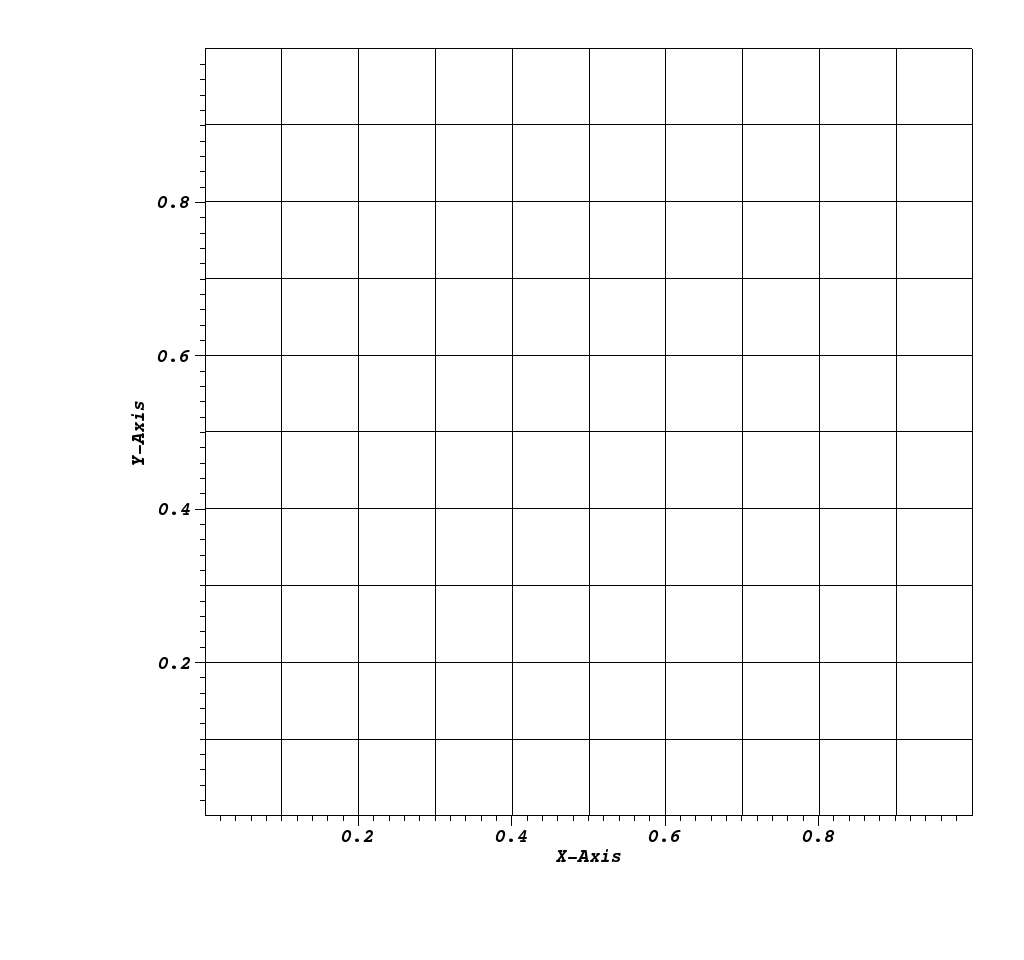
\includegraphics[width=\textwidth]{figures/sec_DSA/IP_cart_mesh.png}
		\caption{}
	\end{subfigure}
	\hfill
	\begin{subfigure}[b]{0.48\textwidth}
		\centering
		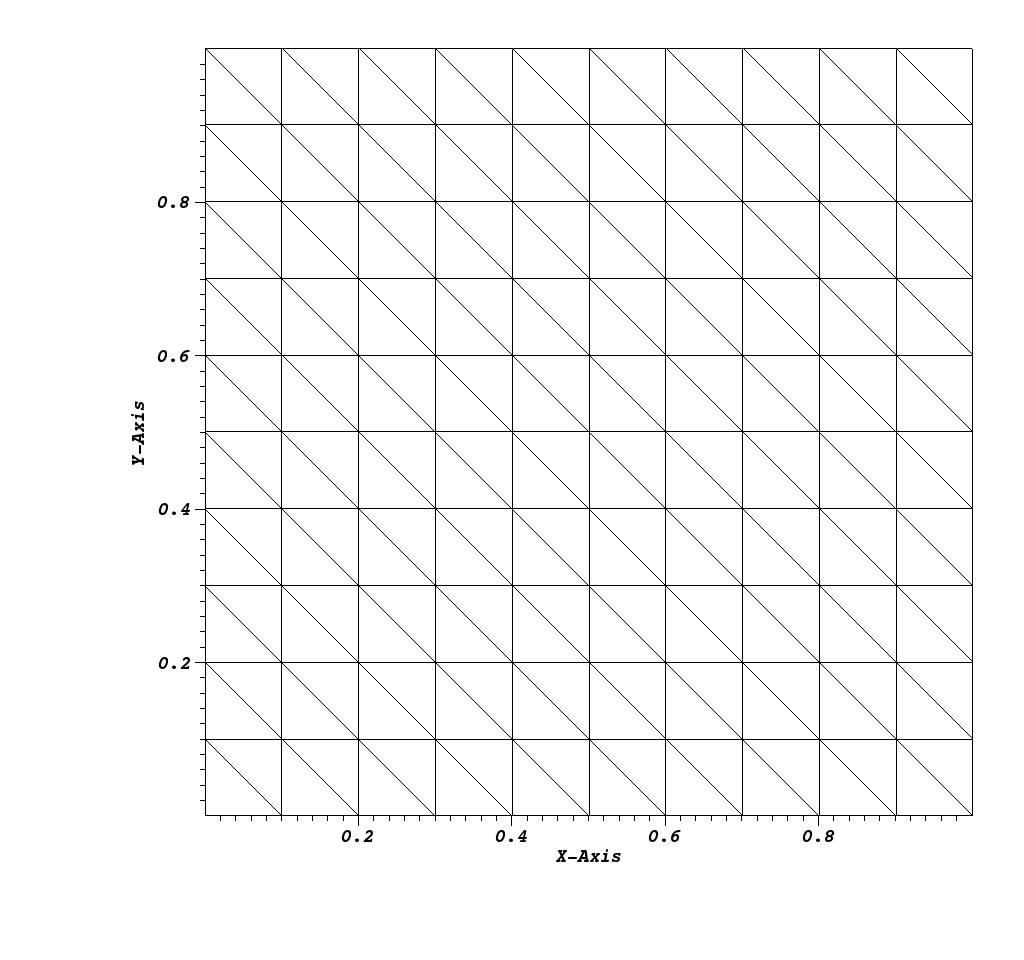
\includegraphics[width=\textwidth]{figures/sec_DSA/IP_tri_mesh.png}
		\caption{}
	\end{subfigure}
\caption{blah}
\end{figure}

\begin{figure}
\centering
\label{fig::IP_coefficient_degradation}
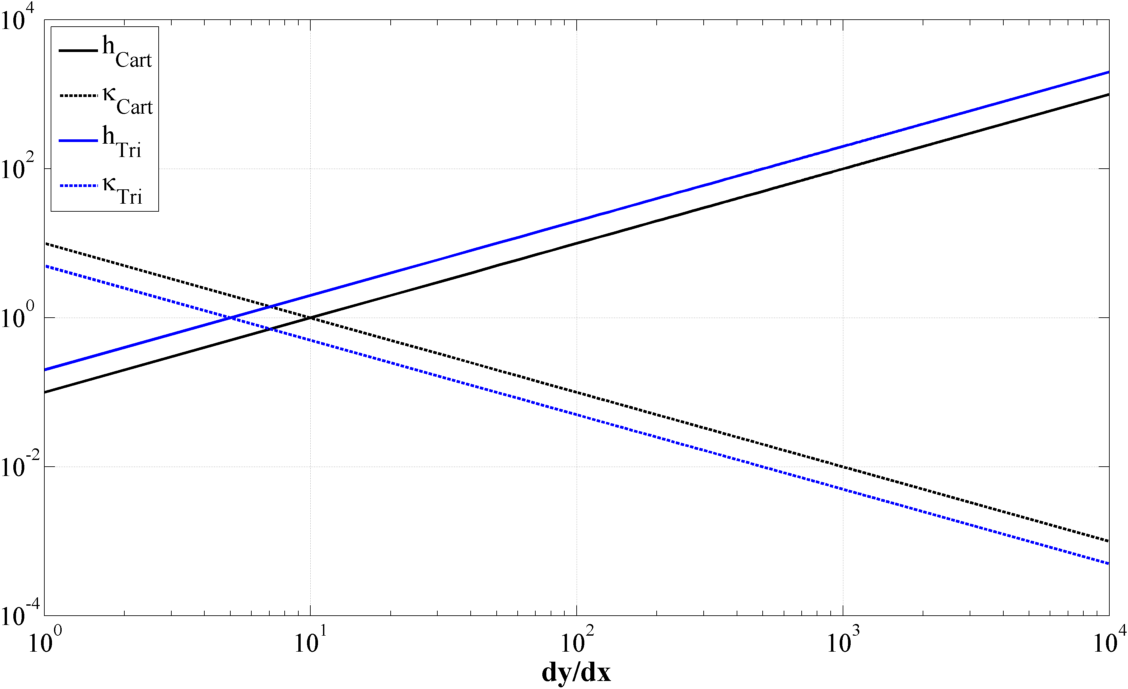
\includegraphics[width=0.8\textwidth]{figures/sec_DSA/IP_penalty_coeff.png}
\caption{Maximum SIP orthogonal projections (solid) and penalty coefficients (dashed) on ordered cartesian (black) and triangular (blue) grids. }
\end{figure}

\begin{equation}
\label{eq::MIP_penalty_term}
\kappa_e^{MIP} = \text{max} \left( \kappa_e^{SIP}, \frac{1}{4} \right)
\end{equation}

%%%%%%%%%%%%%%%%%%%%%%%%%%%%%%%%%%%%%%%%%%%%%%%%%%%
%%%%%%%%%%%%%%%%%%%%%%%%%%%%%%%%%%%%%%%%%%%%%%%%%%%
%%%   Section - MG
%%%%%%%%%%%%%%%%%%%%%%%%%%%%%%%%%%%%%%%%%%%%%%%%%%%
%%%%%%%%%%%%%%%%%%%%%%%%%%%%%%%%%%%%%%%%%%%%%%%%%%%
\section{Multigroup Applications of Diffusion Synthetic Acceleration}
\label{sec::DSA_MG}

\begin{equation}
\label{eq::DSA_MG::mg_trans_op}
{\bf L}_g \Psi_g =  {\bf M} \sum_{g'=1}^{G} {\bf S}_{gg'} \Phi_{g'} + Q_g, \qquad \Phi_g \equiv  {\bf D} \Psi_g
\end{equation}


\begin{equation}
\label{eq::DSA_MG::mg_error_terms}
\delta \Psi_g^{(\ell+1)} \equiv \Psi_g - \Psi_g^{(\ell+1)} \qquad \text{and} \qquad \delta \Phi_g^{(\ell+1)} \equiv  {\bf D} \delta \Psi_g^{(\ell+1)},
\end{equation}

%%%%%%%%%%%%%%%%%%%%%%%%%%%%%%%%%%%%%%%%%%%%%%%%%%%
%%%%%%%%%%%%%%%%%%%%%%%%%%%%%%%%%%%%%%%%%%%%%%%%%%%
%%%   Section - Fourier
%%%%%%%%%%%%%%%%%%%%%%%%%%%%%%%%%%%%%%%%%%%%%%%%%%%
%%%%%%%%%%%%%%%%%%%%%%%%%%%%%%%%%%%%%%%%%%%%%%%%%%%
\section{Fourier Analysis}
\label{sec::DSA_Fourier}

\begin{figure}
\centering
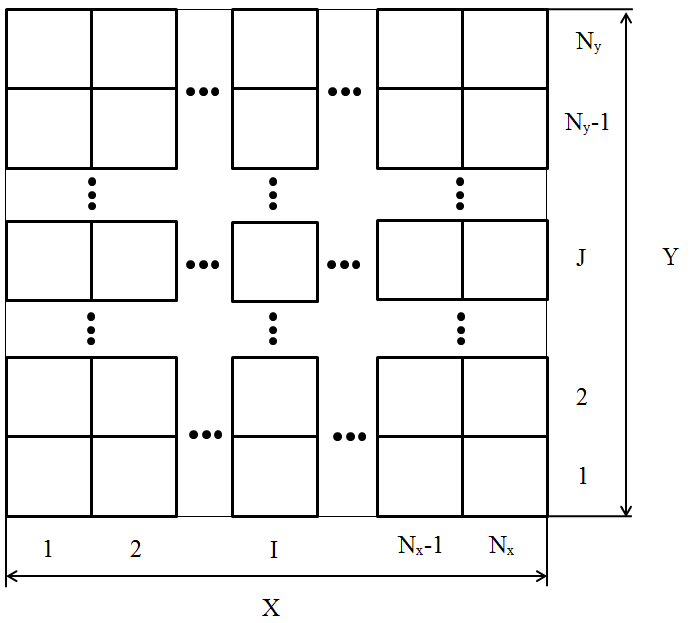
\includegraphics[width=0.60\textwidth]{figures/sec_DSA/fourier_sq_layout.png}
\caption{Fourier domain for 2D quadrilateral cells or an axial slice of 3D hexahedral cells in a regular grid.}
\label{fig::}
\end{figure}

\begin{equation}
\label{eq::fourier_sol}
\begin{aligned}
\Psi_m (\vec{r}) = \hat{\Psi}_m e^{i \vec{\lambda} \cdot \vec{r}}\\
\Phi (\vec{r}) = \hat{\Phi} e^{i \vec{\lambda} \cdot \vec{r}}
\end{aligned}
\end{equation}

\noindent where $i=\sqrt{-1}$

%%%%%%%%%%%%%%%%%%%%%%%%%%%%%%%%%%%%%%%%%%%%%%%%%%%
%%%%%%%%%%%%%%%%%%%%%%%%%%%%%%%%%%%%%%%%%%%%%%%%%%%
%%%   Section - Results
%%%%%%%%%%%%%%%%%%%%%%%%%%%%%%%%%%%%%%%%%%%%%%%%%%%
%%%%%%%%%%%%%%%%%%%%%%%%%%%%%%%%%%%%%%%%%%%%%%%%%%%
\section{Numerical Results}
\label{sec::DSA_Results}

We now present the results showing the efficacy of a discontinuous diffusion form which can be used as a DSA preconditioner for the transport equation discretized over arbitrary grids. We first present the SIP form and how it performs as a pure diffusion solver on unstructured polyhedral grids in Section \ref{sec::DSA_Results_SIP}. We next present the theoretical performance limits of the MIP form as a DSA preconditioner using Fourier Analysis in Section \ref{sec::DSA_Results_Fourier}. We finish by presenting the results of MIP's use as a DSA preconditioner for several different problem types in Section \ref{sec::DSA_Results_MIP}.

%%%%%%%%%%%%%%%%%%%%%%%%%%%%%%%%%%%%%%%%%%%%%%%%%%%
%%%%%%%%%%%%%%%%%%%%%%%%%%%%%%%%%%%%%%%%%%%%%%%%%%%
%%%   SubSection - Thick Diffusive Limit
\subsection{Transport Solutions in the Thick Diffusive Limit}
\label{sec::DSA_Results_TDL}

We present our first numerical example by demonstrating that the various polygonal finite element basis sets satisfy the thick diffusion limit. 


\begin{equation}
\label{eq::BF_Results_TDL_scaling}
\begin{aligned}
	\sigma_t &\rightarrow \frac{\sigma_t}{\epsilon} \\
	\sigma_a &\rightarrow \epsilon \sigma_t\\
	\frac{Q_0}{4 \pi} &\rightarrow \epsilon \frac{Q_0}{4 \pi}
\end{aligned}
\end{equation}

\begin{equation}
\label{eq::BF_Results_TDL_scaled_trans_eq}
\vec{\Omega} \cdot \vec{\nabla} \Psi + \frac{\sigma_t}{\epsilon} \Psi = \sigma_t \left( \frac{1}{\epsilon} - \epsilon   \right)  \frac{\Phi}{4 \pi} + \epsilon \frac{Q_0}{4 \pi}
\end{equation}

\begin{equation}
\label{eq::BF_Results_TDL_scaled_diff_eq}
\epsilon \vec{\nabla} \cdot \frac{1}{3 \sigma_t}  \vec{\nabla} \Phi + \epsilon \sigma_t \Phi =  \epsilon Q_0
\end{equation}

\begin{equation}
\label{eq::BF_Results_TDL_normalized_eqs}
\begin{aligned}
\vec{\Omega} \cdot \vec{\nabla} \Psi + \frac{1}{\epsilon} \Psi &=  \left( \frac{1}{\epsilon} - \epsilon   \right)  \frac{\Phi}{4 \pi} +  \frac{\epsilon}{4 \pi} \\
\frac{\epsilon}{3} {\nabla}^2 \Phi &+ \epsilon  \Phi =  \epsilon 
\end{aligned}
\end{equation}

%%%%%%%%%%%%%%%%%%%%%%%%%%%%%%%%%%%%%%%%%%%%%%%%%%%
%%%   SubSection - SIP Results
\subsection{SIP used as a Diffusion Solver}
\label{sec::DSA_Results_SIP}

We first wish to know how an interior penalty form of the diffusion equation will perform on unstructured polyhedral grids. We will perform this analysis with a stand-alone MATLAB code. The polyhedral mesh types for this analysis are presented in Section \ref{sec::DSA_Results_SIP_Geometry}. 

\begin{enumerate}
	\item A purely-linear solution to determine if linear basis functions will span the solution space;
	\item The Method of Manufactured Solutions to test basis function convergence rates;
\end{enumerate}

\noindent in Sections \ref{sec::DSA_Results_SIP_Linear} and \ref{sec::DSA_Results_SIP_MMS}, respectively. 

%%%%%%%%%%%%%%%%%%%%%%%%%%%%%%%%%%%%%%%%%%%%%%%%%%%
%%%   SubSubSection - SIP Results = Geometry
\subsubsection{Geometry Specification for the SIP Problems}
\label{sec::DSA_Results_SIP_Geometry}

For this work in

\begin{figure}
\centering
	\begin{subfigure}[b]{0.5\textwidth}
		\centering
		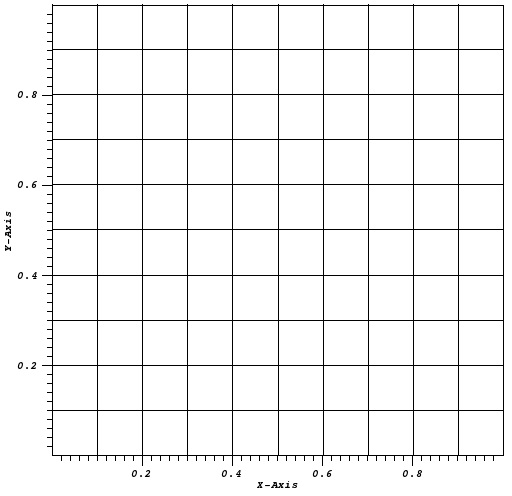
\includegraphics[width=0.82\textwidth]{figures/sec_DSA/SIP_cart_mesh.png}
		\caption{}
	\end{subfigure}
	\vfill
	\begin{subfigure}[b]{0.45\textwidth}
		\centering
		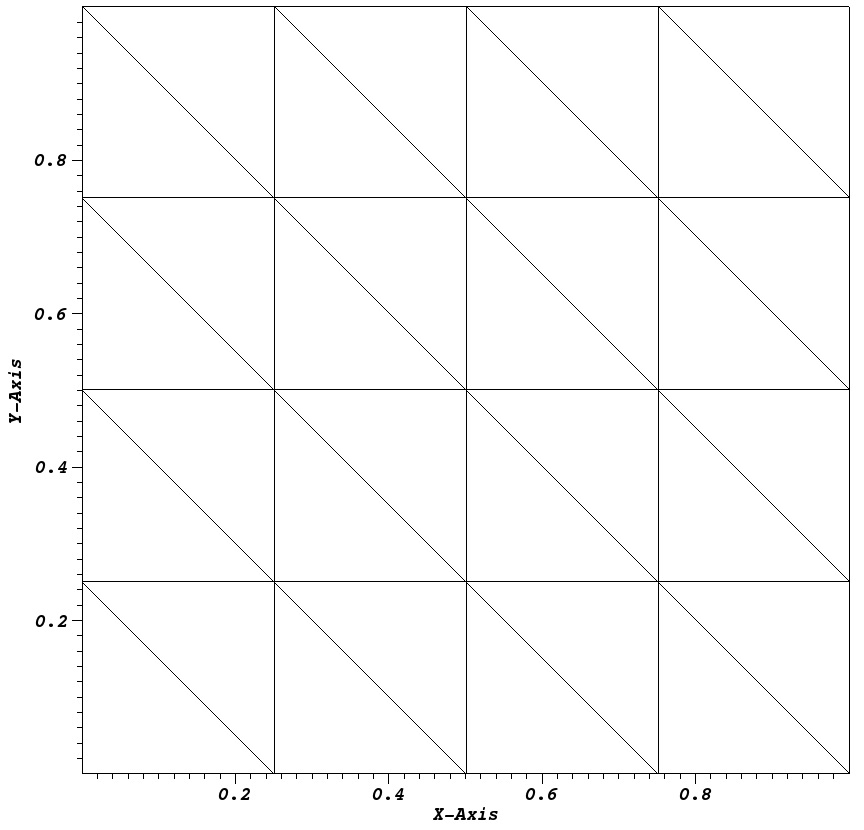
\includegraphics[width=0.85\textwidth]{figures/sec_DSA/SIP_tri_mesh.png}
		\caption{}
	\end{subfigure}
	\hfill
	\begin{subfigure}[b]{0.45\textwidth}
		\centering
		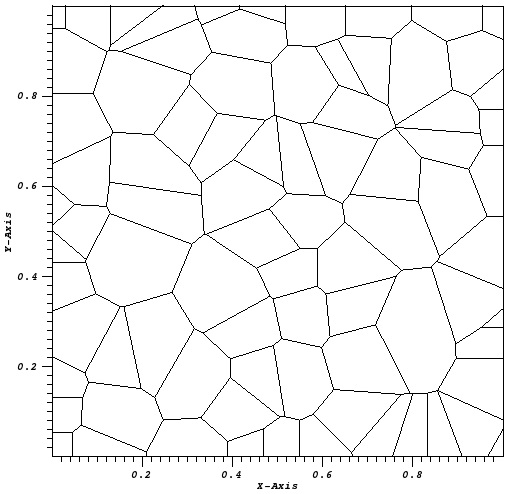
\includegraphics[width=0.85\textwidth]{figures/sec_DSA/SIP_poly_mesh.png}
		\caption{}
	\end{subfigure}
	\vfill
	\begin{subfigure}[b]{0.45\textwidth}
		\centering
		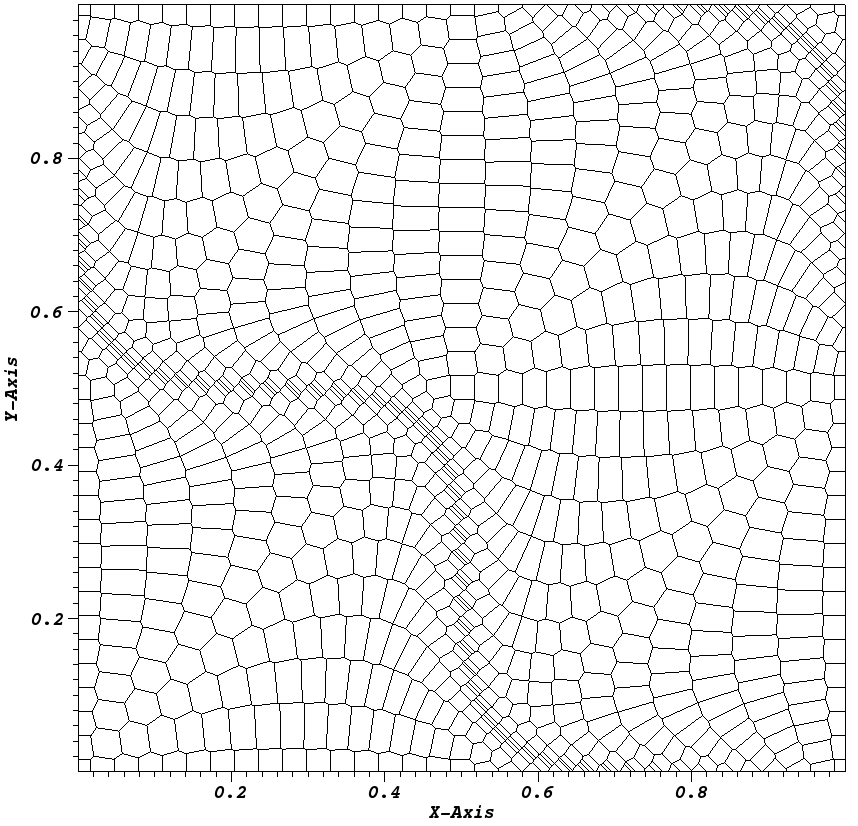
\includegraphics[width=0.85\textwidth]{figures/sec_DSA/SIP_sine_poly_mesh.png}
		\caption{}
	\end{subfigure}
	\hfill
	\begin{subfigure}[b]{0.45\textwidth}
		\centering
		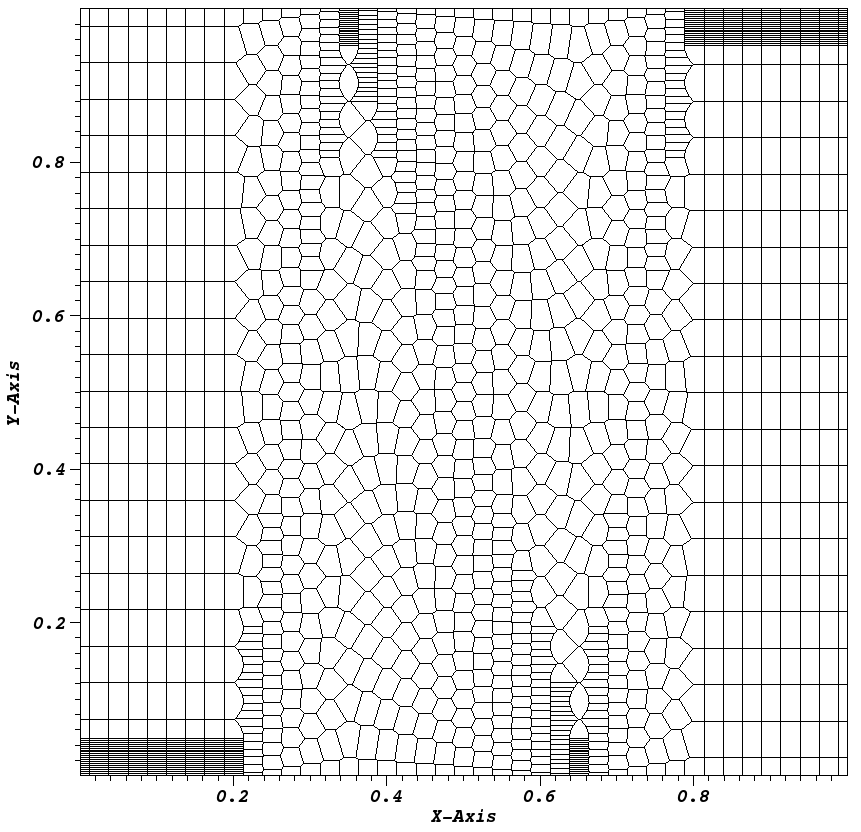
\includegraphics[width=0.85\textwidth]{figures/sec_DSA/SIP_z_poly_mesh.png}
		\caption{}
	\end{subfigure}
\caption{Axial slices of the different mesh types: (a) cartesian, (b) ordered triangles, (c) random polygons, (d) sinusoidal polygons, and (e) polygonal z-mesh.}
\label{fig::SIP_mesh_slices}
\end{figure}

\begin{figure}
\centering
	\begin{subfigure}[b]{0.5\textwidth}
		\centering
		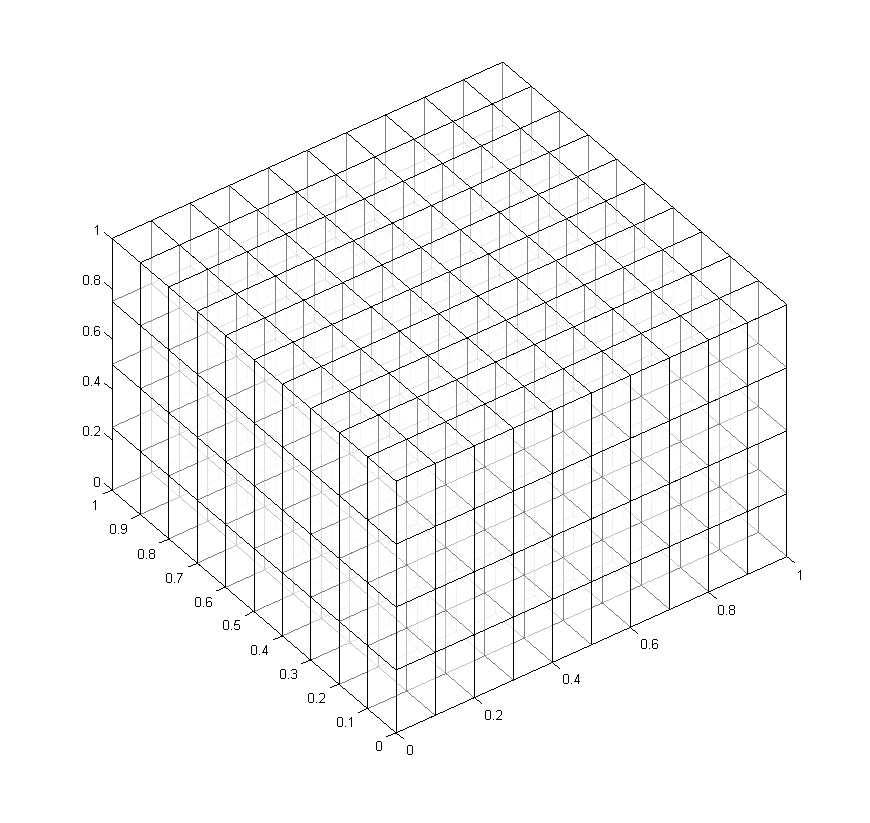
\includegraphics[width=0.82\textwidth]{figures/sec_DSA/SIP_cart_extruded_mesh.png}
		\caption{}
	\end{subfigure}
	\vfill
	\begin{subfigure}[b]{0.45\textwidth}
		\centering
		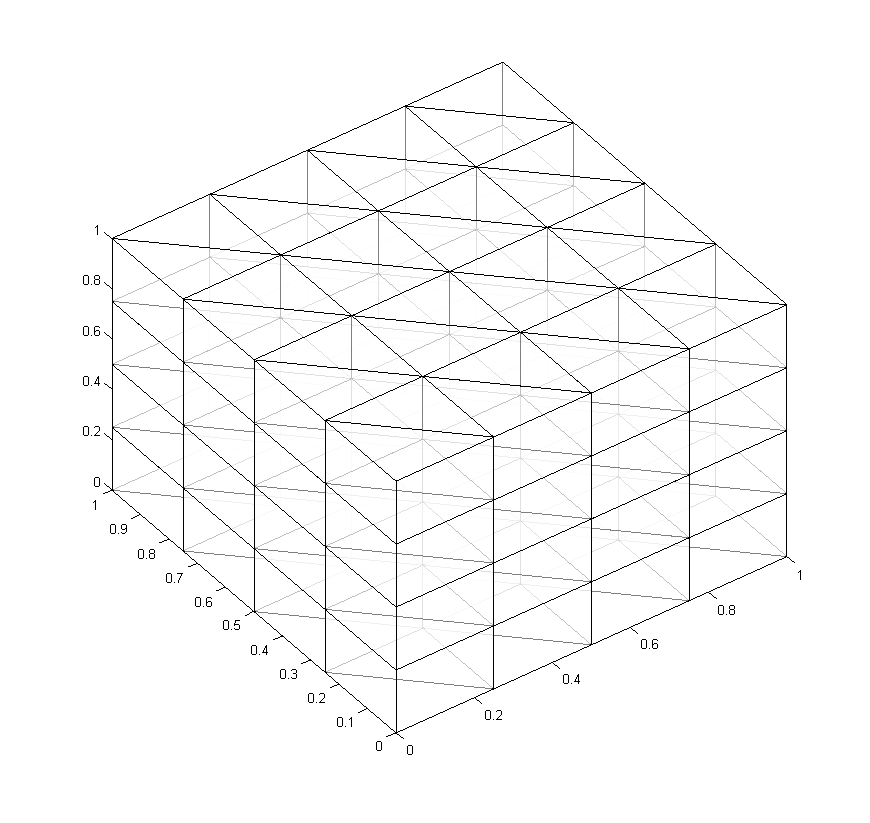
\includegraphics[width=0.85\textwidth]{figures/sec_DSA/SIP_tri_extruded_mesh.png}
		\caption{}
	\end{subfigure}
	\hfill
	\begin{subfigure}[b]{0.45\textwidth}
		\centering
		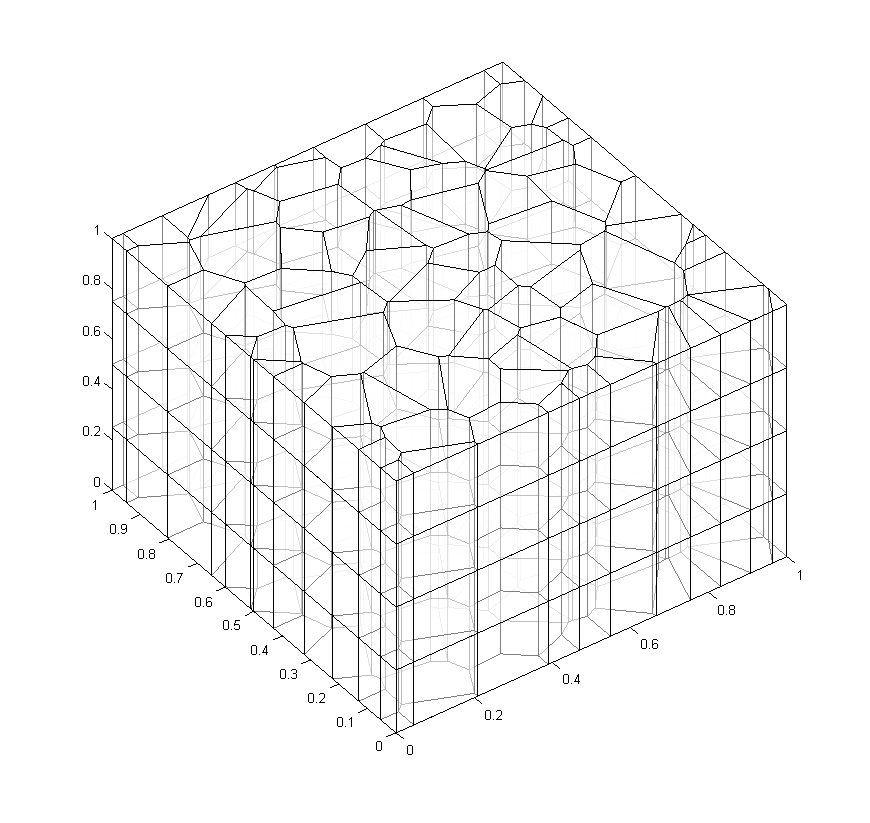
\includegraphics[width=0.85\textwidth]{figures/sec_DSA/SIP_poly_extruded_mesh.png}
		\caption{}
	\end{subfigure}
	\vfill
	\begin{subfigure}[b]{0.45\textwidth}
		\centering
		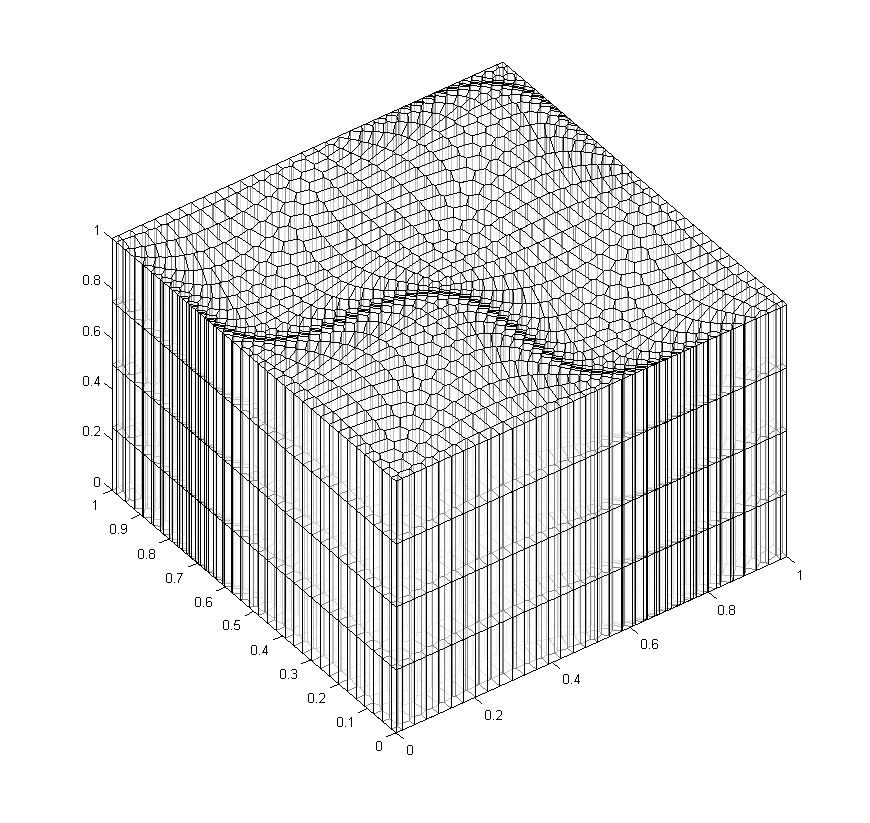
\includegraphics[width=0.85\textwidth]{figures/sec_DSA/SIP_sine_poly_extruded_mesh.png}
		\caption{}
	\end{subfigure}
	\hfill
	\begin{subfigure}[b]{0.45\textwidth}
		\centering
		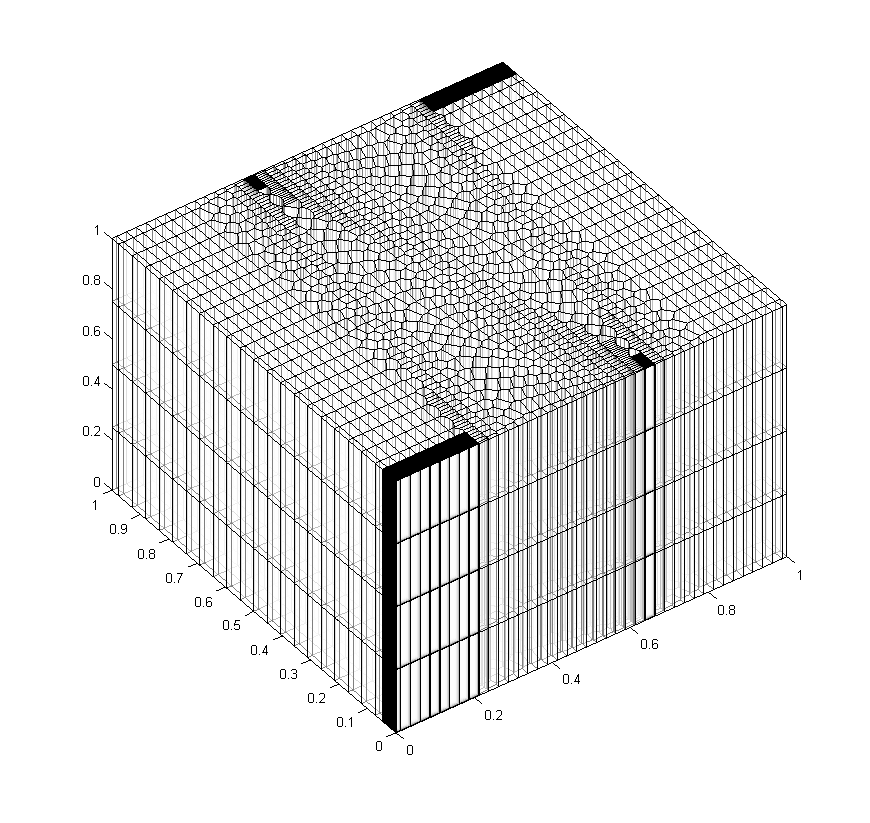
\includegraphics[width=0.85\textwidth]{figures/sec_DSA/SIP_z_poly_extruded_mesh.png}
		\caption{}
	\end{subfigure}
\caption{Extrusion of the different mesh types: (a) cartesian, (b) ordered triangles, (c) random polygons, (d) sinusoidal polygons, and (e) polygonal z-mesh.}
\label{fig::SIP_mesh_extruded}
\end{figure}

%%%%%%%%%%%%%%%%%%%%%%%%%%%%%%%%%%%%%%%%%%%%%%%%%%%
%%%   SubSubSection - SIP Results = Linear
\subsubsection{Purely-Linear Solution}
\label{sec::DSA_Results_SIP_Linear}

We first test SIP by enforcing a sytem that yields a purely-linear solution. Linear finite elements should then theoretically fully-span the solution space. We can achieve this mathematically by setting the cross-section and right-hand-source terms to zero, $\sigma = Q = 0$. Robin boundary conditions are imposed on opposite faces in 1 dimension, with homogeneous Neumann boundary conditions on all other faces. If the Robin boundaries are chosen in the y-direction, with $y \in (0,L)$, then the analytical solution for the problem will be 

\begin{equation}
\label{eq::mms_lin_solution}
\Phi(x,y,z) = \frac{4 J^{inc}}{L + 4D} \left(  L + 2 D - y \right),
\end{equation}

\noindent with the following boundary conditions in the y-direction:

\begin{equation}
\label{eq::mms_lin_bcs}
\begin{aligned}
\Phi - 2D \partial_y \Phi = & 4 J^{inc}, \qquad & \forall (x,z),y=0 \\
\Phi + 2D \partial_y \Phi = & 0, \qquad & \forall (x,z),y=L
\end{aligned}.
\end{equation}

\begin{figure}
\centering
	\begin{subfigure}[b]{0.5\textwidth}
		\centering
		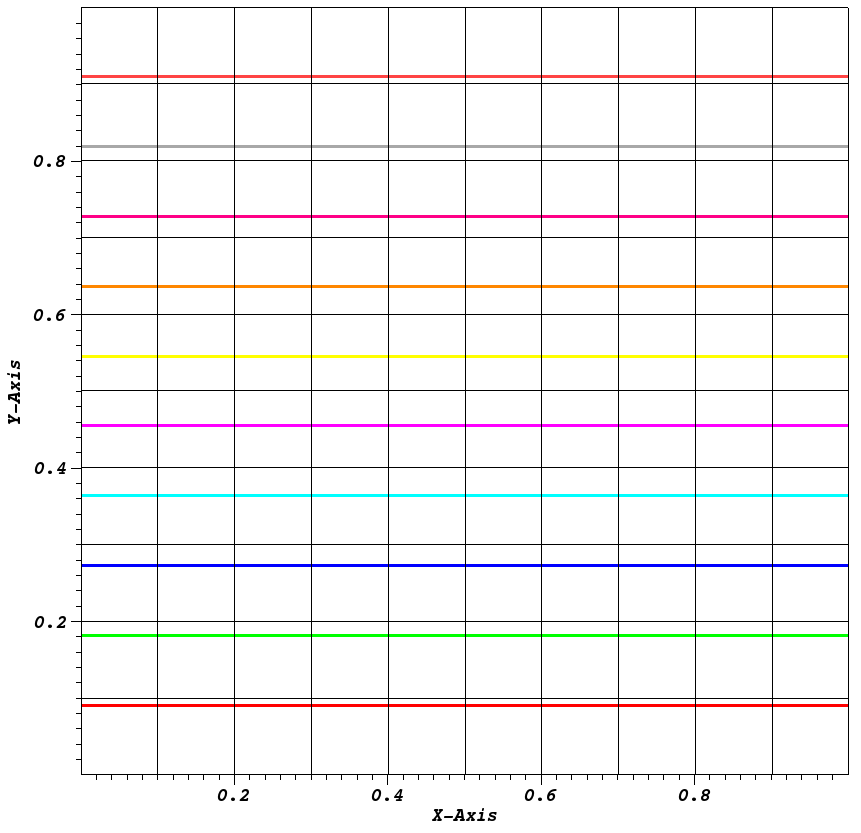
\includegraphics[width=0.82\textwidth]{figures/sec_DSA/SIP_cart_lin_contour.png}
		\caption{}
	\end{subfigure}
	\vfill
	\begin{subfigure}[b]{0.45\textwidth}
		\centering
		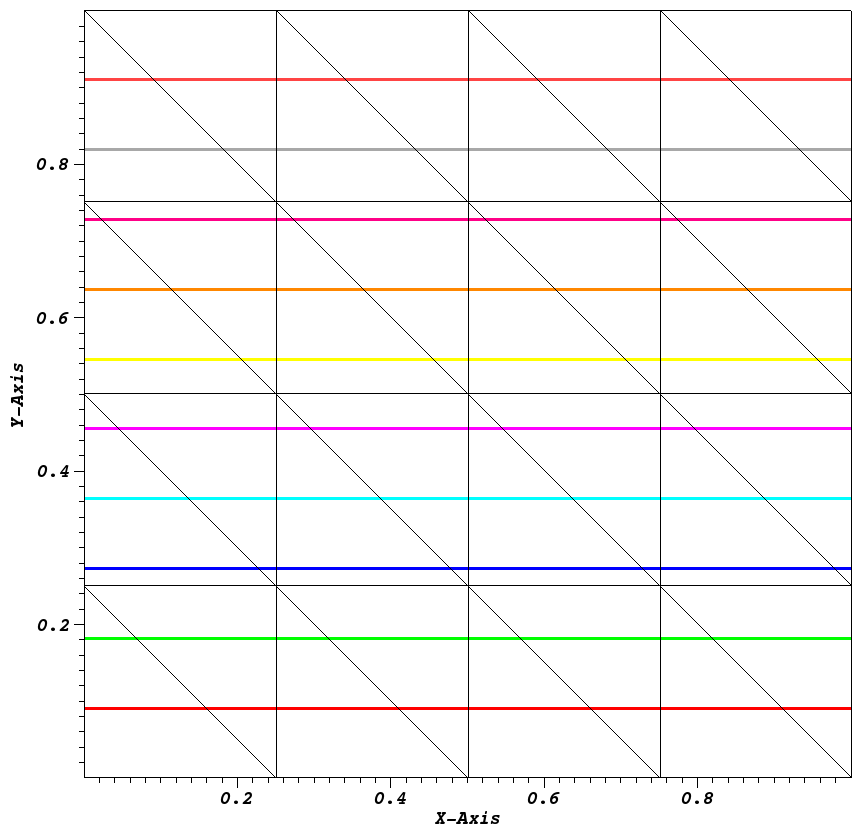
\includegraphics[width=0.85\textwidth]{figures/sec_DSA/SIP_tri_lin_contour.png}
		\caption{}
	\end{subfigure}
	\hfill
	\begin{subfigure}[b]{0.45\textwidth}
		\centering
		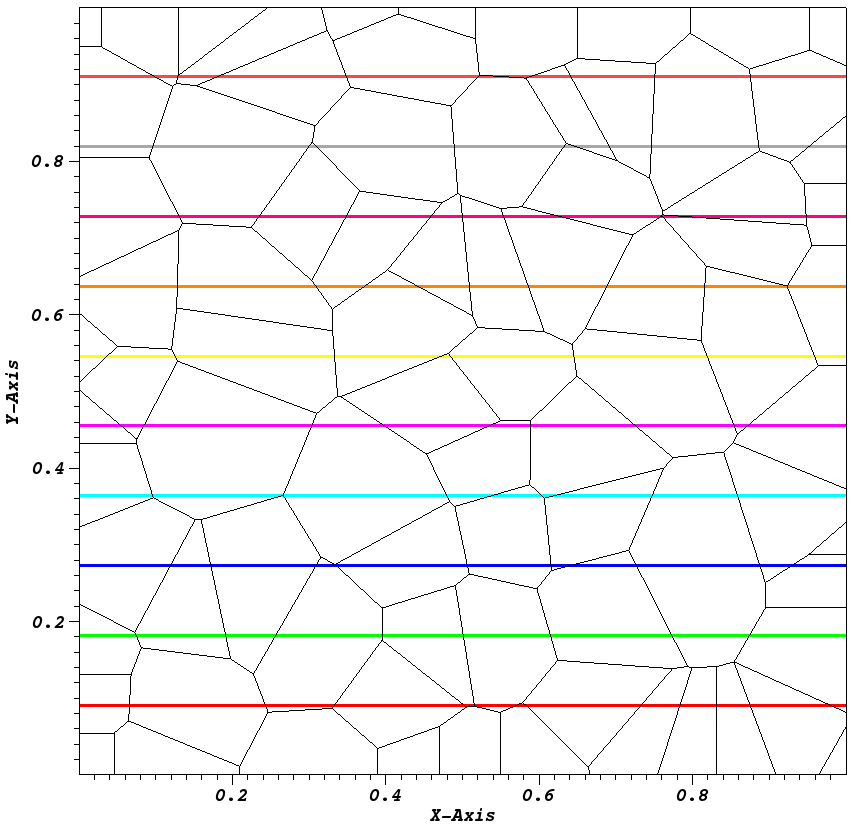
\includegraphics[width=0.85\textwidth]{figures/sec_DSA/SIP_poly_lin_contour.png}
		\caption{}
	\end{subfigure}
	\vfill
	\begin{subfigure}[b]{0.45\textwidth}
		\centering
		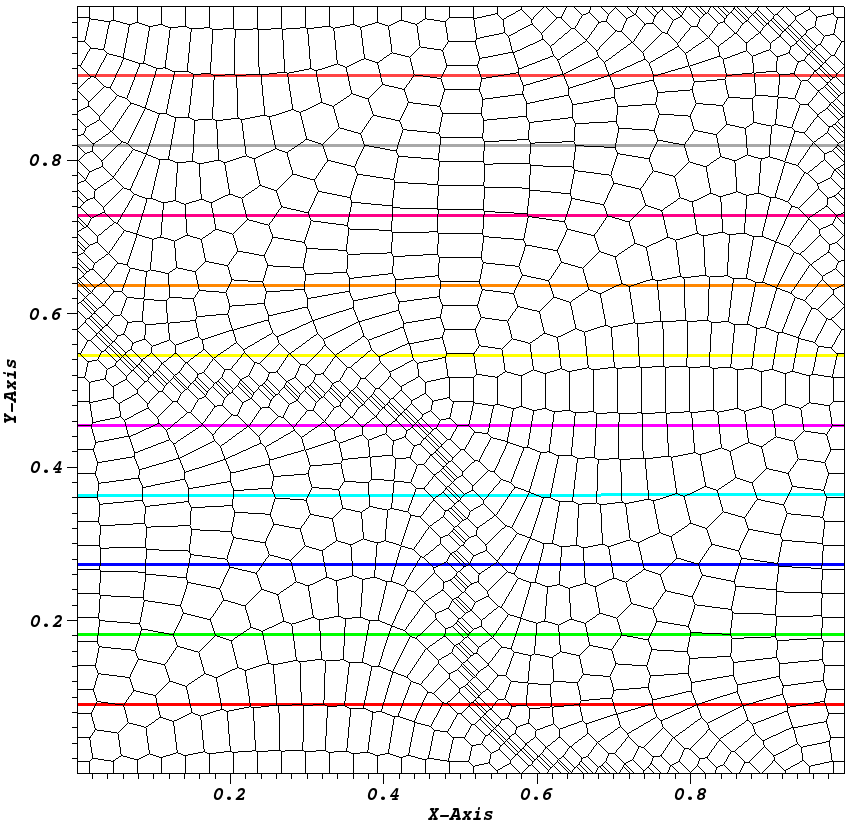
\includegraphics[width=0.85\textwidth]{figures/sec_DSA/SIP_sine_poly_lin_contour.png}
		\caption{}
	\end{subfigure}
	\hfill
	\begin{subfigure}[b]{0.45\textwidth}
		\centering
		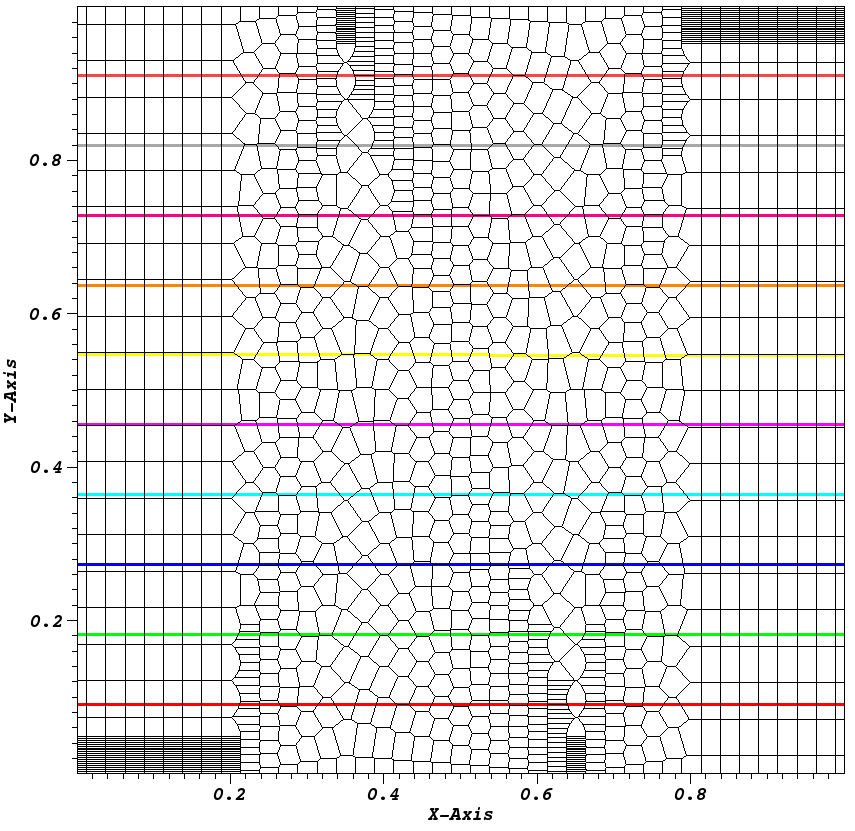
\includegraphics[width=0.85\textwidth]{figures/sec_DSA/SIP_z_poly_lin_contour.png}
		\caption{}
	\end{subfigure}
\caption{Axial slice showing the contours for the linear solution of the different mesh types: (a) cartesian, (b) ordered triangles, (c) random polygons, (d) sinusoidal polygons, and (e) polygonal z-mesh.}
\label{fig::SIP_mesh_slices}
\end{figure}

%%%%%%%%%%%%%%%%%%%%%%%%%%%%%%%%%%%%%%%%%%%%%%%%%%%
%%%   SubSubSection - SIP Results = MMS
\subsubsection{Method of Manufactured Solutions}
\label{sec::DSA_Results_SIP_MMS}

\begin{equation}
\label{eq::SIP_quad_mms_solution}
\begin{aligned}
\Phi^{quad} (x,y,z) = x(1-x)y(1-y)z(1-z) 
\end{aligned}
\end{equation}

\begin{equation}
\label{eq::SIP_gauss_mms_solution}
\begin{aligned}
\Phi^{gauss} (x,y,z) = \Phi^{quad} (x,y,z) \exp(- (\vec{r} - \vec{r}_0) \cdot (\vec{r} - \vec{r}_0)^{T}  )
\end{aligned}
\end{equation}


\begin{figure}
\centering
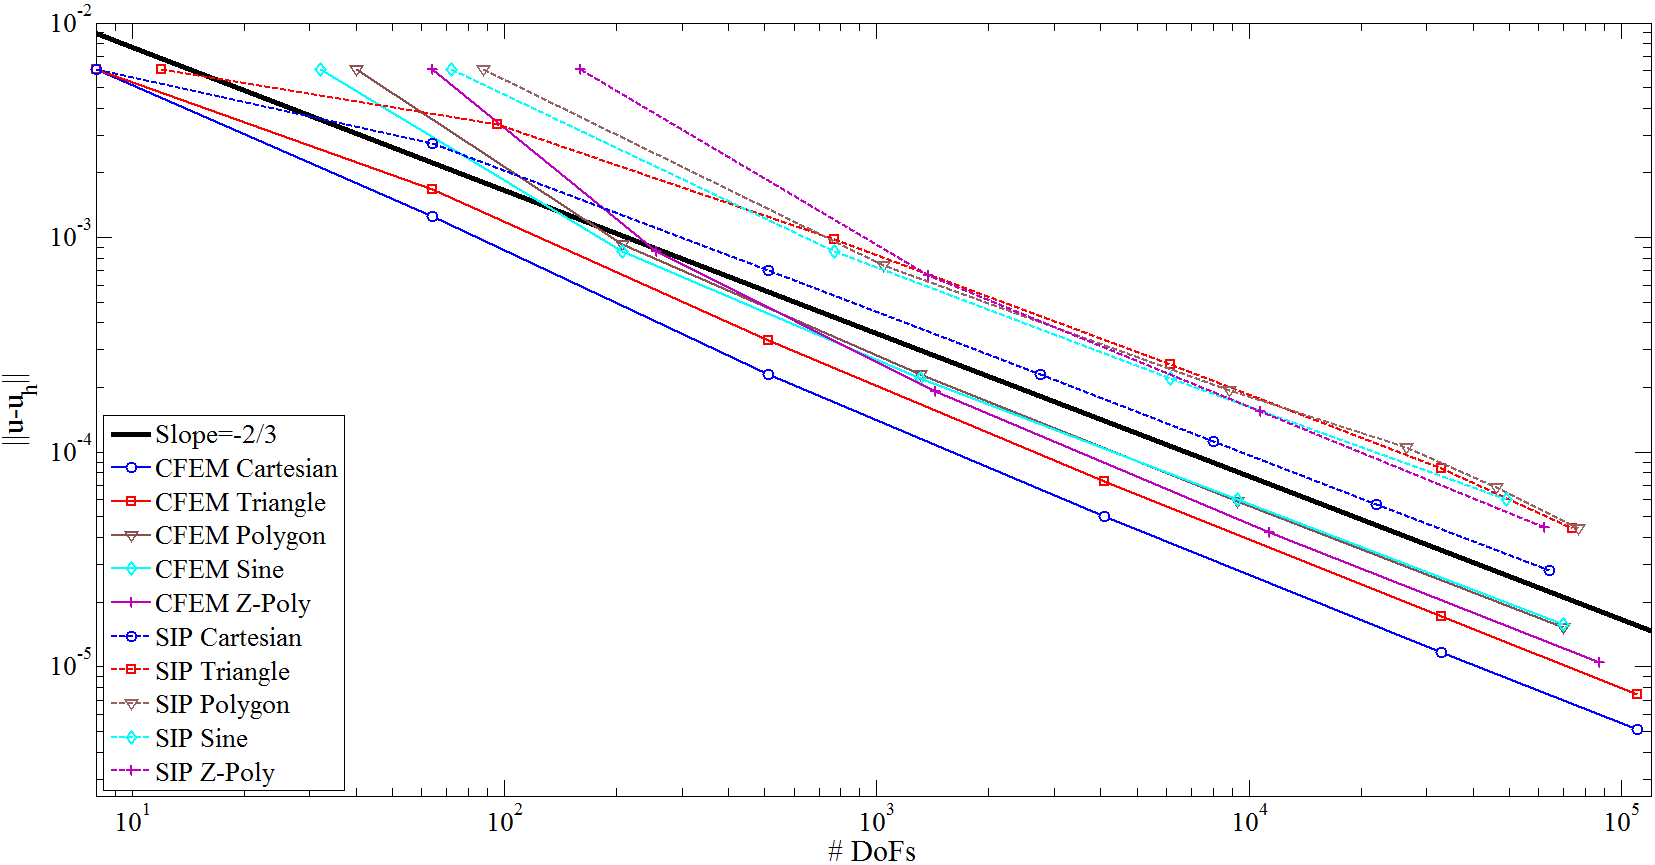
\includegraphics[width=\textwidth]{figures/sec_DSA/SIP_mms_3d_quad_full_paint.png}
\caption{blah}
\label{fig::SIP_mms_quad_error_plot}
\end{figure}

\begin{figure}
\centering
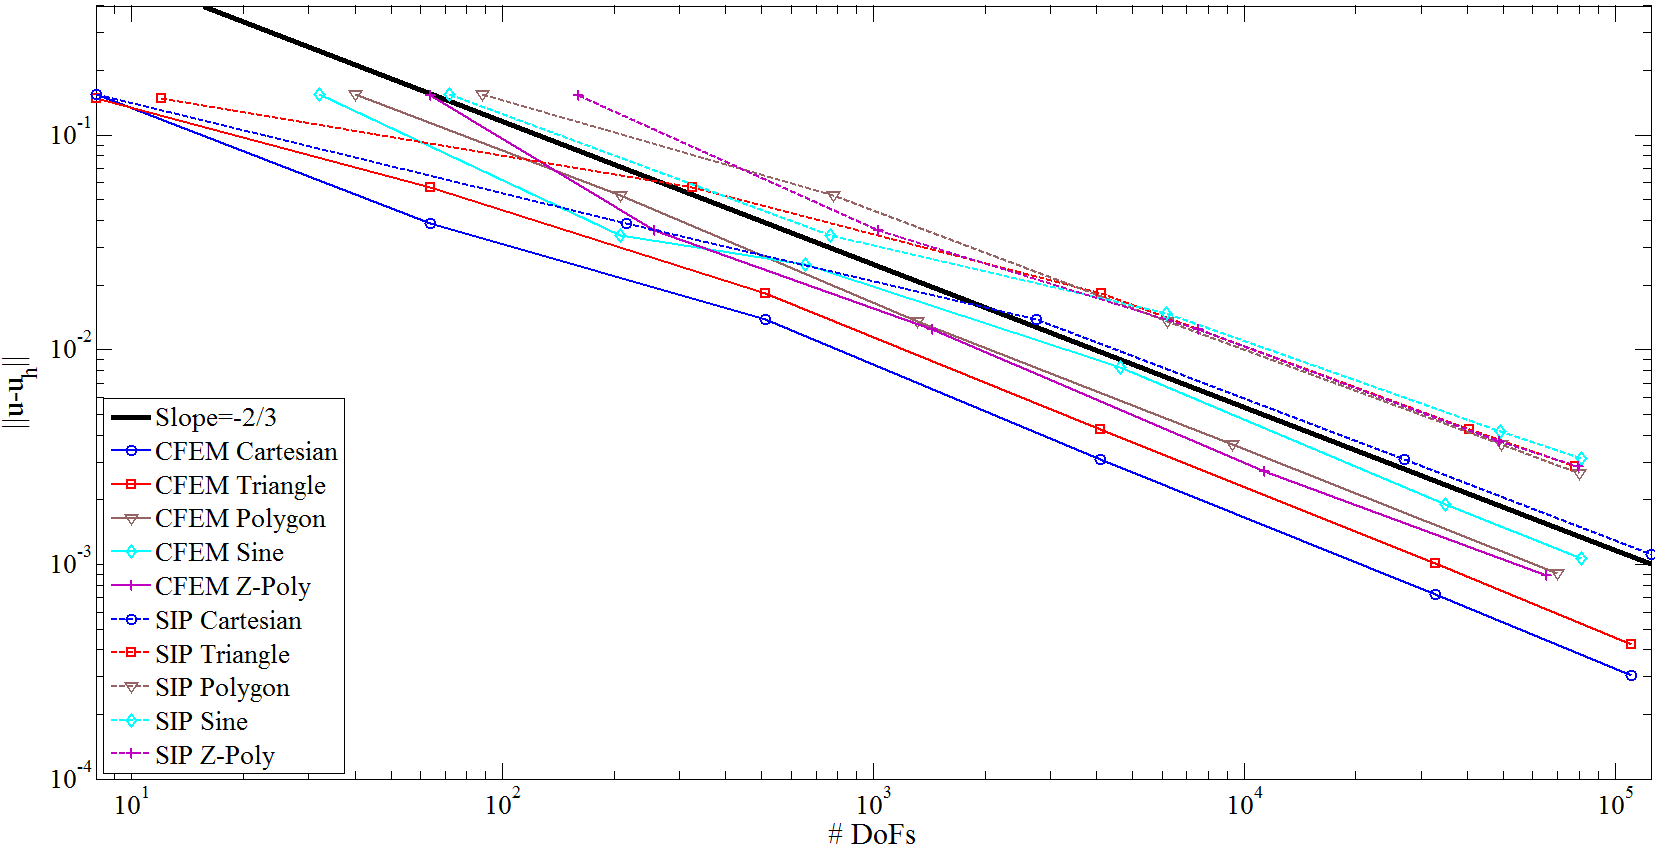
\includegraphics[width=\textwidth]{figures/sec_DSA/SIP_mms_3d_gauss_full_paint.png}
\caption{blah}
\label{fig::SIP_mms_gauss_error_plot}
\end{figure}


%%%%%%%%%%%%%%%%%%%%%%%%%%%%%%%%%%%%%%%%%%%%%%%%%%%
%%%%%%%%%%%%%%%%%%%%%%%%%%%%%%%%%%%%%%%%%%%%%%%%%%%
%%%   SubSection - Fourier Results
\subsection{Fourier Analysis}
\label{sec::DSA_Results_Fourier}

%%%%%%%%%%%%%%%%%%%%%%%%%%%%%%%%%%%%%%%%%%%%%%%%%%%
%%%   SubSubSection - Fourier Results = Homogeneous Medium
\subsubsection{Homogeneous Medium Case}
\label{sec::DSA_Results_Fourier_Homo}

\begin{figure}
\centering
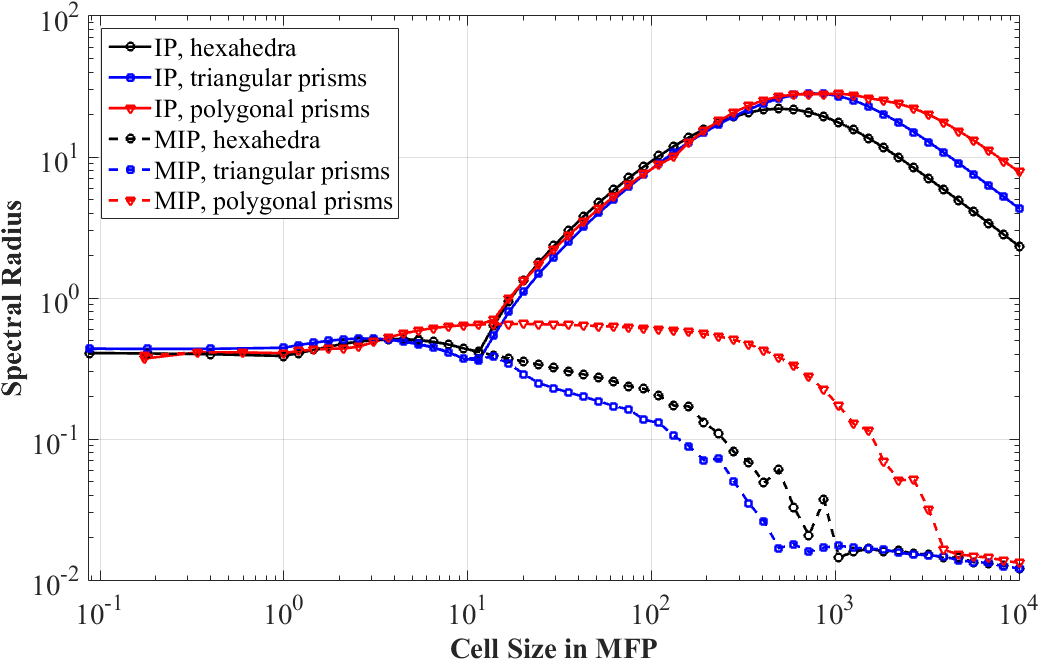
\includegraphics[width=\textwidth]{figures/sec_DSA/IP,MIP_V_hex,tri,poly_LS8_C=4.png}
\caption{blah}
\label{fig::IP_MIP_Homo_LS8_C4}
\end{figure}

%%%%%%%%%%%%%%%%%%%%%%%%%%%%%%%%%%%%%%%%%%%%%%%%%%%
%%%   SubSubSection - Fourier Results = PHI
\subsubsection{Periodic Horizontal Interface (PHI) Problem}
\label{sec::DSA_Results_Fourier_PHI}


%%%%%%%%%%%%%%%%%%%%%%%%%%%%%%%%%%%%%%%%%%%%%%%%%%%
%%%%%%%%%%%%%%%%%%%%%%%%%%%%%%%%%%%%%%%%%%%%%%%%%%%
%%%   SubSection - MIP Results
\subsection{MIP Results}
\label{sec::DSA_Results_MIP}

We have given a theoretical basis for MIP's stability using Fourier Analysis in Section \ref{sec::DSA_Results_Fourier}. In this Section, we provide numerical results of DSA preconditioning of the Discontinuous $S_N$ Transport Equation. We first provide 

%%%%%%%%%%%%%%%%%%%%%%%%%%%%%%%%%%%%%%%%%%%%%%%%%%%
%%%   SubSubSection - MIP Results = Simple Homo Domain
\subsubsection{Simple Homogeneous Problem Results}
\label{sec::DSA_Results_MIP_Homo}

%%%%%%%%%%%%%%%%%%%%%%%%%%%%%%%%%%%%%%%%%%%%%%%%%%%
%%%   SubSubSection - MIP Results = Hetero
\subsubsection{Heterogenous Problem Results}
\label{sec::DSA_Results_MIP_Hetero}


%%%%%%%%%%%%%%%%%%%%%%%%%%%%%%%%%%%%%%%%%%%%%%%%%%%
%%%%%%%%%%%%%%%%%%%%%%%%%%%%%%%%%%%%%%%%%%%%%%%%%%%
%%%   Section - Conclusions
%%%%%%%%%%%%%%%%%%%%%%%%%%%%%%%%%%%%%%%%%%%%%%%%%%%
%%%%%%%%%%%%%%%%%%%%%%%%%%%%%%%%%%%%%%%%%%%%%%%%%%%
\section{Conclusions}
\label{sec::DSA_conclusions}

In this chapter, we have presented a discontinuous form of the diffusion equation, known as the Modified Interior Penalty Method (MIP), which can be applied to the discontinuous finite element form of the transport equation as a DSA preconditioner. 
